% !TeX root = ../main.tex
% Add the above to each chapter to make compiling the PDF easier in some editors.

\chapter{Design}\label{chapter:design}
\section{Trust, Usability and Privacy}
In any platform, we expect a certain level of trust from each participant, may it be from the service provider or its consumer. How this trust is created can have many different sources. But the main reason a person or organization can be trusted is because of accountability. Companies with a strong market presence have the public's trust since they have been present for a longer period of time and can't just disappear overnight
 Consequently, they can be held accountable for their actions. Today, Microsoft, Google, Amazon, and Facebook, for instance, are seen as trustworthy to a certain degree. But this trust is not invulnerable. Lies and secrecy can damage trust. Keeping the public uninformed about severe data breaches or selling sensitive data to third parties without their knowledge and permission has strained the public trust in recent years.
% Todo: \cite[Facebook Cambridge Analytica]

Even if the trust is in place, we as consumers require privacy. If we can guarantee anonymity, however, we can also guarantee privacy, as re-identification should be impossible at that point.
% Todo: \cite[Dictionary]

As chapter 2 has shown, it is a hard task to anonymize big data sets, as quasi-identifiers can be used to infer new information using linking attacks. So one way to achieve anonymity would be to strip away all attributes that could be used in another data set.

Here we hit a wall with the usability of the data itself. Cynthia Dwork says "de-identified data isn't,"
% Todo: \cite[Cynthia Dwork]
meaning that either that the data itself is not de-identified because of possible reconstruction of the data is not data anymore because it is not useful for analysis purposes. We see data itself is only as useful as its relationships.

So there is a need to find a way to find a balance between trust, usability, and privacy. Due to the limited scope of the thesis and trust being a vast research subject, we focus on the privacy of the crowd and the usability of their collected data. We assume that all participating devices and servers can be trusted, and possible adversaries only have access to the published end results.

\section{Approaches}
As mentioned before, there are advantages and disadvantages to Simon van Endern's system, and we explore how we can implement improvements and if they would be feasible with the current state of the art or if another alternative has to be chosen.

\subsection{Simon van Endern}
The proposed architecture implemented in his thesis was using a centralized approach with a distributed storage solution. The model can be seen in figure \ref{fig:simon_original}.

\begin{figure}[htpb]
  \centering
  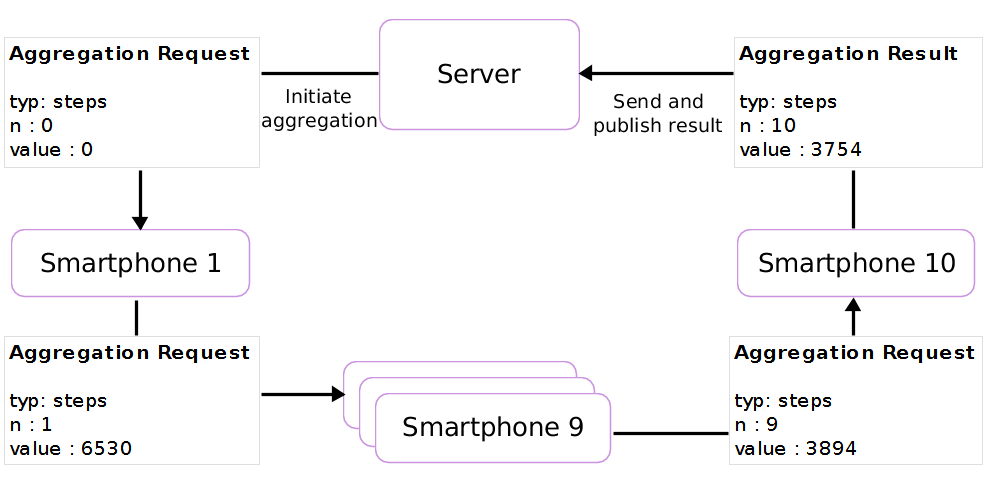
\includegraphics[width=0.8\textwidth]{figures/simon_original.png}
  \caption{Simon van Endern's original architecture.} \label{fig:simon_original}
\end{figure}

In his thesis, he eliminates the need for a central database, by collecting and storing raw data directly on the users' smartphone, creating a distributed database. This gives each participant a lot of control over their own data, just by deleting the application they are able to opt-out of future data analyses.

In his original idea, the mobile phones would use peer-to-peer technology to forward the aggregation requests and finally send the data to the server for publication. But because of the lack of available technology, he opted to use the central server as an intermediary to send from mobile phone to mobile phone. To keep the data confidential and ensure anonymity from the server, he uses RSA and AES encryption. To forward the data to the next device, he implemented a polling solution. The application periodically asks for a new aggregation request targeted at the device from the server. If one is present, it fetches the request over the REST API, and after adding its own data, it posts it back to the server targeting the next device.
In the finite scope, he managed to implement three aggregation types:

\begin{itemize}
    \item Average number of steps over the course of a day for participants. 
    \item Average time spent on an activity (walking, running, in a vehicle or on a bicycle).
    \item Average number of steps of a participant during the test period. 
\end{itemize}

We examined his work and discovered a few flaws that we might be able to improve on. We will look into possible solutions to make the architecture more efficient, scalable, secure, and privacy-preserving. 

\subsection{Expanded Approach}
Simon van Endern's original idea, as is, can hardly be scaled because of the nature of its forwarding chain. Adding \(n\) new devices creates a linear time complexity of \(\mathcal{O}(n)\) and space complexity of \(\mathcal{O}(n^2)\). For every device added, the aggregation takes up to an additional 15 minutes, and the data fetched and sent is the data of all previous devices combined, making it quite a burden on participant's data plan depending on their position in the chain. 

To make the architecture more scalable, we propose to parallelize these chains by building multiple groups for the aggregation, as shown in figure [X]. With \(m\) groups, adding \(n\) devices, now only creates a time complexity of \(\mathcal{O}(\dfrac{n}{m})\) and space complexity of \(\mathcal{O}((\dfrac{n}{m})^2)\). So choosing the right \(m\) would change linear and quadratic to constant potential growth. 

We also intend to implement local differential privacy because to protect the collected data from information leakage.

Additionally, to avoid unnecessary constant polling, we will explore some P2P frameworks that can send data directly to the next target device and cut down on forwarding delays.

In order to extend the aggregation options, we add the two following two types:
\begin{itemize}
    \item number of participants that were at a location in a specific time period
    \item General location of all participants in a location at a specific time
\end{itemize}

